\documentclass{standalone}
\usepackage[svgnames]{xcolor}
\usepackage{tikz}
\usepackage[english]{babel}
\usepackage[T1]{fontenc}
\usepackage[utf8]{inputenc}
\usepackage{microtype}

\tikzstyle{legend}=[inner sep=0pt,black]
\tikzstyle{peers}=[draw,circle,black]
%,bottom color=DodgerBlue, top color= white,
% \tikzstyle{pose}=[line width=2.5pt,color=LawnGreen]
% \tikzstyle{nege}=[line width=2.5pt,color=FireBrick]
\tikzstyle{pose}=[line width=2.5pt,solid,black]
\tikzstyle{nege}=[line width=2.5pt,dashed,black]
\tikzstyle{c1}=[fill=DodgerBlue]
\tikzstyle{c2}=[fill=Orange]
\tikzstyle{c3}=[fill=SpringGreen]
% \tikzstyle{disa}=[line width=3pt,dashed]
% \tikzstyle{disa}=[line width=3pt,red]
\tikzstyle{label}=[scale=1]
\begin{document}
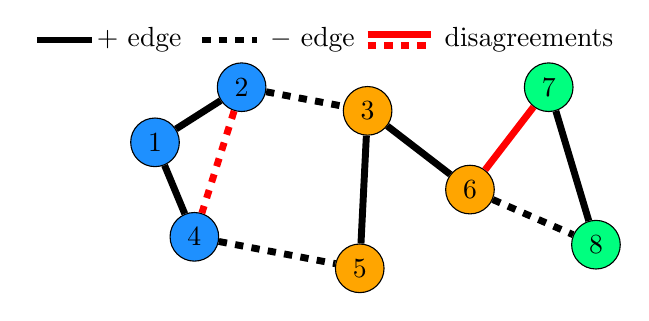
\begin{tikzpicture}[auto]
	% \foreach \place/\name in {%
	% {(0,4)/1}, {(1.6,5)/2}, {(0.2,2.5)/4},
	% {(2.2,3)/3}, {(2.1,1)/5}, {(3.5,2)/6},
	% {(4.5,4)/7}, {(5.1,1.3)/8}}
    % \node[peers] (\name) at \place {\name};
	\foreach \place/\name in { {(-0.5,2.6)/1}, {(0.6,3.3)/2}, {(0,1.4)/4}}
    \node[peers,c1] (\name) at \place {\name};
\foreach \place/\name in {{(2.2,3)/3}, {(2.1,1)/5}, {(3.5,2)/6}}
    \node[peers,c2] (\name) at \place {\name};
    \foreach \place/\name in  {{(4.5,3.3)/7}, {(5.1,1.3)/8}}
    \node[peers,c3] (\name) at \place {\name};
	\foreach \source/\dest in {1/2, 1/4, 3/5, 3/6, 7/8}
	% \draw[pose] (\source) edge node[label]{$+$} (\dest);
	\draw[pose] (\source) edge  (\dest);

  \foreach \source/\dest in {2/3,4/5,6/8}
    % \draw[nege] (\source) edge node[label]{$-$} (\dest);
    \draw[nege] (\source) edge  (\dest);

	\draw[pose] (-2,3.9) edge (-1.3,3.9) node (poslegend) {};
	\node[legend] at (-0.7,3.9) {$+$ edge};
	\draw[nege] (0.1,3.9) edge (0.8,3.9) node (neglegend) {};
    \node[legend] at (1.5,3.9) {$-$ edge};
	\draw[pose,red] (2.2,3.97) edge (3,3.97);
	\draw[nege,red] (2.2,3.83) edge (3,3.83);
	\node[legend] at (4.25,3.9) {disagreements};

    \draw[pose,red] (6) edge  (7);
    \draw[nege,red] (2) edge  (4);
	% \draw[pose] (6) edge node[label]{$+$} (7);
	% \draw[nege] (2) edge node[label]{$-$} (4);

\end{tikzpicture}
\end{document}

